\documentclass{article}

\usepackage[final]{nips_2017}

\usepackage[utf8]{inputenc} % allow utf-8 input
\usepackage[T1]{fontenc}    % use 8-bit T1 fonts
\usepackage{hyperref}       % hyperlinks
\usepackage{url}            % simple URL typesetting
\usepackage{booktabs}       % professional-quality tables
\usepackage{amsfonts}       % blackboard math symbols
\usepackage{nicefrac}       % compact symbols for 1/2, etc.
\usepackage{microtype}      % microtypography
\usepackage{graphicx}

\title{Pun Detection and Location\\Group C}

\author{
   Shantanu Karnwal \texttt{shantanu.karnwal@colorado.edu} \\
   \And Amir Kashipazha \texttt{amirhossein.kashipazha@colorado.edu} \\
   \And Brandon Boylan-Peck \texttt{brbo9266@colorado.edu} \\
   \And Cathlyn Stone \texttt{cathlyn.stone@colorado.edu} \\
   \And Kenneth Hunter Wapman \texttt{kennethwapman@colorado.edu} \\
}

\begin{document}

\maketitle

\begin{abstract}
	Pun identification and location are challenging natural language processing 
	tasks. We implemented several algorithms for both, with results which 
	were competitive with the systems presented in the SemEval conference, where
	those tasks were originally defined.
\end{abstract}

%%%%%%%%%%%%%%%%%%%%%%%%%%%%%%%%%%%%%%%%%%%%%%%%%%%%%%%%%%%%%%%%%%%%%%%%%%%%%%%
% Problem Description
%%%%%%%%%%%%%%%%%%%%%%%%%%%%%%%%%%%%%%%%%%%%%%%%%%%%%%%%%%%%%%%%%%%%%%%%%%%%%%%

\section{Overview}
A pun is a form of wordplay within the class of textual phenomena involving
ambiguity where multiple meanings of a word or set of words are played upon to
create a rhetorical effect. They occur in many domains: in advertising, puns
are used to connect a product with a desirable quality; in literature, puns are
used to add a level of meaning and implication; in conversation, puns add humor
to the topic at hand.

Understanding a pun often requires the integration of information from a large
number of contexts; syntax, morphology, semantics, and pragmatics, and context
can all come into play. There are many types of puns:

\begin{itemize}
	\item{\textbf{Homographic}: A pun involving two words whose spellings are
		the same but have different meanings.
		\begin{center}
		\emph{I used to be a banker but I lost \textbf{interest}.}
		\end{center}
	}
	\item{\textbf{Heterographic}: A pun involving two or more words which sound
		alike but are spelled differently. Sometimes termed `homophonic'.
		\begin{center}
		\emph{Two construction workers had a \textbf{stairing} contest.}
		\end{center}
	}
	\item{\textbf{Compound}: A sentence containing two or more puns.
		\begin{center}
		\emph{Why can a man never starve in the Great Desert? Because he can
		eat the sand which is there. But what brought the sandwiches there?
		Why, Noah sent Ham, and his descendants mustered and bred.} - Richard Whately
		\end{center}
	}
	\item{\textbf{Visual}: A pun realized by an image. See figure \ref{fig:visual_pun}\footnote{\url{https://digitalsynopsis.com/design/punny-pixels-illustrated-puns-visual-wordplay/}}.
	}
\end{itemize}

\begin{figure}
\centering
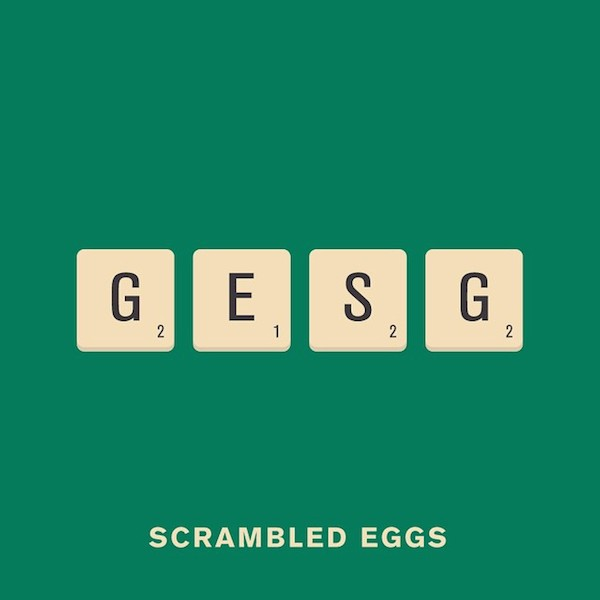
\includegraphics[width=5cm]{figures/visual_pun.jpg}
\caption{A visual Pun.}\label{fig:visual_pun}
\end{figure}

We focused on two types: homographic puns and heterographic puns. 

\subsection{Motivation}

It would be desirable for machines to be able to identify, comprehend, and
generate puns for a number of reasons:

\begin{itemize}
	\item A pun generator could facilitate slogan generation, which would be
		useful in advertising and dialogue agents.
	\item A pun identifier could be used to improve machine translations, where
		literal translation of puns rarely conveys the original text's message.
	\item A pun comprehension system would be helpful for large-scale textual
		analyses of the kind increasingly being employed in the digital
		humanities.
\end{itemize}

We worked on two related tasks: pun detection and pun location.

\subsection{Dataset}

We trained and tested our algorithms on the test sets used to appraise the
competing systems in SemEval2017 Task 7. The dataset for each of the tasks we
worked on was split into two parts: homographic and heterographic. We modified
the characteristics of these datasets to address some issues we found. Namely,
the original datasets for the detection tasks for both heterographic and
homographic puns had a pun/non-pun split of 70/30. The non-pun sentences for
each type of pun were, however, non-overlapping, so we simply modified each pun
type's dataset to include \emph{all} non-puns from either dataset, giving us a
more even ratio of pun/non-pun. In addition to looking at each dataset
individually, we also combined these datasets to look at it either as a binary
classification task with both types of puns given the same label, or as a
multi-class classification task with the different types of puns given
different labels, but running with all the data for both types.

%%%%%%%%%%%%%%%%%%%%%%%%%%%%%%%%%%%%%%%%%%%%%%%%%%%%%%%%%%%%%%%%%%%%%%%%%%%%%%%
% Pun Detection
%%%%%%%%%%%%%%%%%%%%%%%%%%%%%%%%%%%%%%%%%%%%%%%%%%%%%%%%%%%%%%%%%%%%%%%%%%%%%%%

\section{Pun Detection}\label{pun_detection}

Pun detection is a binary classification problem: given a sequence of words (a
sentence), determine whether or not that sentence contains a pun. 

We tried a number of different approaches to this problem, but found that the
best approach was a Bidirectional LSTM.

\subsection{Baseline: Multinomial Naive Bayes}

A random approach to this task will have a $50\%$ of being correct.
However, we wanted to determine whether we could do better than random with a
simple classifier. To that end, we implemented a simple Multinomial Naive Bayes
classifier. 

\subsection{Linear SVM}

We implemented a linear SVM and trained it using Stochastic Gradient Descent.
The intuition behind this was that an SVM would be able to incorporate arbitrary
features, and that the data would be linearly separable with the right features.
This approach worked quite well, but was slightly less effective than our neural
net approach.

\subsubsection{Feature Comparison}

We tried to improve the Linear SVM's performance by including a variety of
features (Table \ref{tab:List_of_features}), as well as using different
combinations of those features.  Features were added to the code one by one to
find whether they improve accuracy. In general, accuracy improved with the
addition of more features.

We determined which combinations of features would improve the algorithm the
most using a heuristic based approach to select the features to include in
combinations. Testing all combinations of features was not feasible: with 16
features and 65535 combinations of those features, testing each one at a runtime
of 60 seconds per run would have taken 1092 hours. After identifying 11
features (0-10 in table \ref{tab:List_of_features}), we ran a brute-force search
of the 2047 combinations (over both the heterographic and homographic datasets)
of those features to determine which was best.

\begin{table}
\caption{Features by Index}\label{tab:List_of_features} 
\begin{center}
\begin{tabular}{l l l l} 
\toprule
\textbf{\#} &\textbf{Feature Name}		& \textbf{\#} &	\textbf{Feature Name}\\
\midrule
0	&	Lesk Algorithm					& 8		&	Idiom is in Pun or Not\\
1	&	Pos								& 9		&	Antonyms is in Pun or Not\\
2	&	tfidf							& 10	&	Homonym is in Pun or Not\\
3	&	Embeddings						& 11	&	Bigram\\
4	&	Unigram							& 12	&	Trigram\\
5	&	Number of Homophone in Pun		& 13	&	Positives\\
6	&	Number of Each Homophone in Pun & 14	&	Negatives\\
7	&	Homophone is in Pun or Not		& 15	&	All or First Caps\\
\bottomrule
\end{tabular}
\end{center}
\end{table}

\begin{figure}
  \centering
  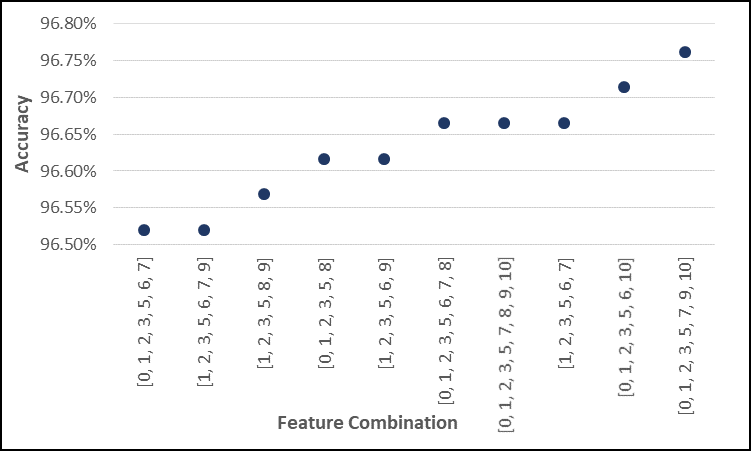
\includegraphics[width=8cm]{figures/Accuracy_on_Training_Set_for_Homographic_Pun.png}
  \caption{Homographic Pun Feature Comparison Training Set Accuracy}\label{fig:ACC_Train_Homo}
\end{figure}

\begin{figure}
  \centering
  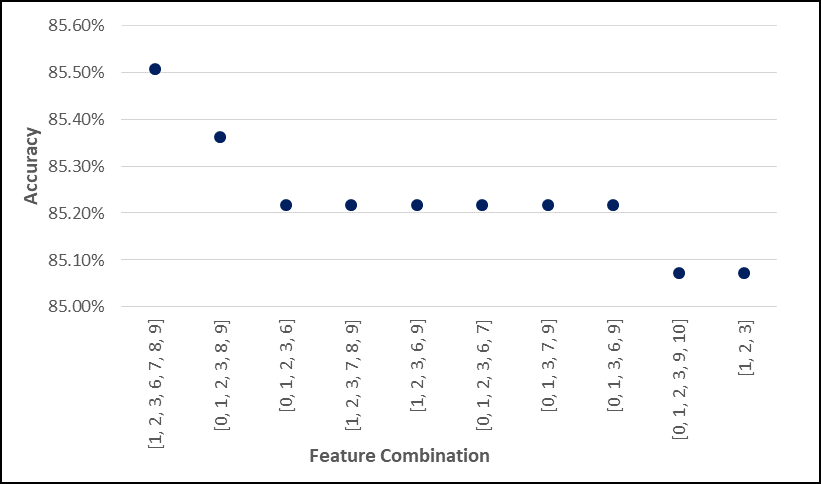
\includegraphics[width=8cm]{figures/Accuracy_on_Test_Set_for_Homographic_Pun.png}
  \caption{Homographic Pun Feature Comparison Test Set Accuracy}\label{fig:ACC_Test_Homo}
\end{figure}

\begin{figure}
  \centering
  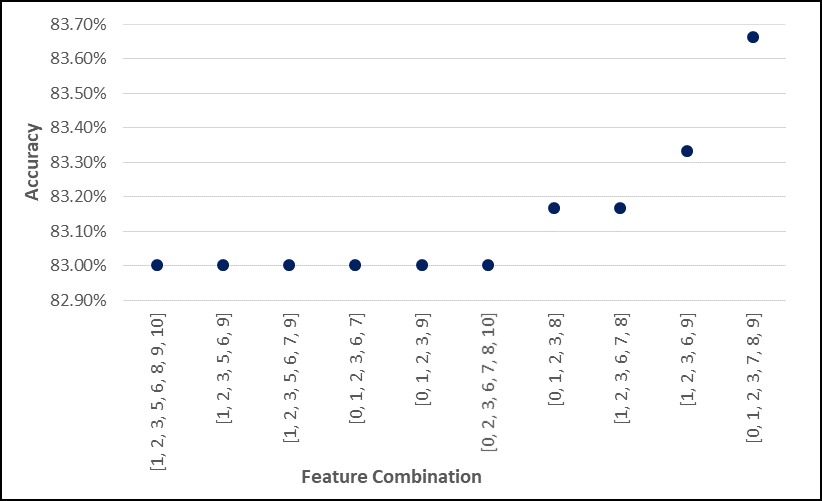
\includegraphics[width=8cm]{figures/Accuracy_on_Test_Set_for_Heterographic_Pun.png}
  \caption{Heterographic Pun Feature Comparison Test Set Accuracy}\label{fig:ACC_Test_Hetero}
\end{figure}

\begin{figure}
  \centering
  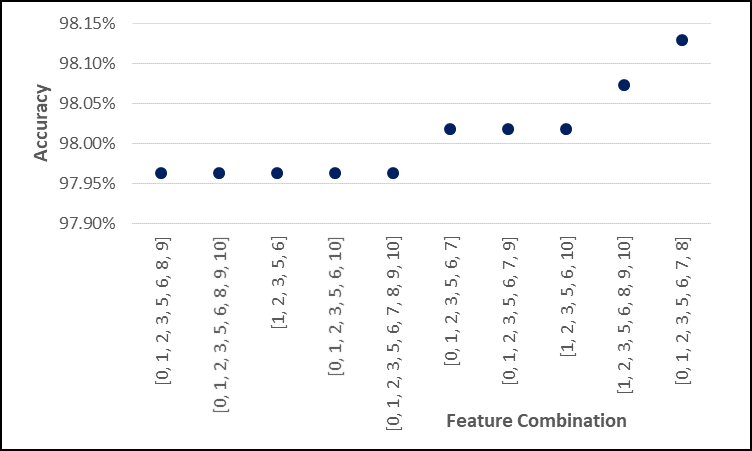
\includegraphics[width=8cm]{figures/Accuracy_on_Training_Set_for_Heterographic_Pun.png}
  \caption{Heterographic Pun Feature Comparison Training Set Accuracy}\label{fig:ACC_Train_Hetero}
\end{figure}

\subsection{Bidirectional LSTM}

Despite having a fairly small dataset, we decided to try a neural net on the
problem. We chose an LSTM because of its ability to deal with variable-sentence
lengths, as (somewhat obviously) our dataset featured sentences of different
lengths. This was our most effective approach. We used glove embeddings with a
length of 300. The intuition behind using a bidirectional LSTM as opposed to a
monodirectional one was that, because pun words are often at the end of the
sentence, processing the back of the sentence first might prime the network to
detect the pun more effectively.

%%%%%%%%%%%%%%%%%%%%%%%%%%%%%%%%%%%%%%%%%%%%%%%%%%%%%%%%%%%%%%%%%%%%%%%%%%%%%%%
% Pun Location
%%%%%%%%%%%%%%%%%%%%%%%%%%%%%%%%%%%%%%%%%%%%%%%%%%%%%%%%%%%%%%%%%%%%%%%%%%%%%%%
\section{Pun Location}
\label{pun_location}

Pun location is a less straightforward task than pun detection: given a set of
words known to contain a pun, identify the pun word. Though this problem is less
amenable to traditional machine learning algorithms, it can be rephrased to be
more similar to one: for each word in the sentence, determine the likelihood
that that word is a pun given the rest of the sentence. Then, output the word
which is most likely to be a pun based on the output of the previous search.  A
random approach to this dataset does not work particularly well; it will have an
accuracy of about 1 divided by the average length of the sentence.
 
\subsection{Baseline}

We implemented a \textbf{Heuristic Decision Tree} model to locate a pun word.
The intuition behind this model was that much of the time, the pun word is
located in the second half of the sentence, and are often involved in an
`interesting' semantic, syntactic, or morphological relationship with another
word: many are antonyms, homophones, homonyms or involved in an idiom. If none
of these relationships obtain, the last word in the sentence is output.

\begin{figure}[h!]
\centering
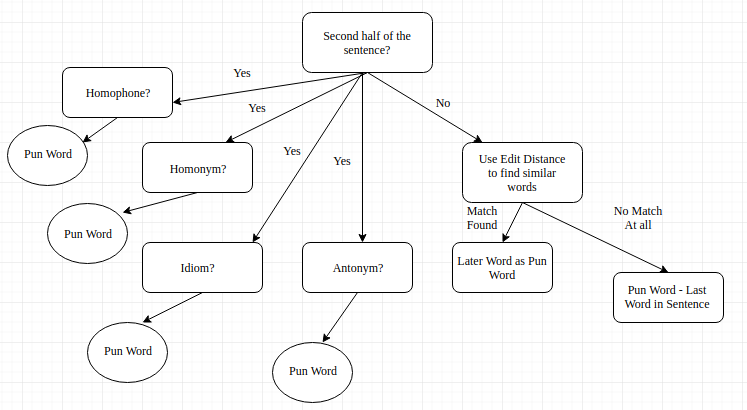
\includegraphics[width=90mm]{figures/decision_tree.png}
\caption{Heuristic Decision Tree Classifier}
\label{fig:method}
\end{figure}

\subsection{Bidirectional LSTM}

We implemented a Bidirection LSTM but treated the problem as a sequence labeling
task, again using 300-length glove embeddings as our word representation. We
then took the maximum prediction of that sequence and used that as the index of
the most likely word. This approach was competitive for the homographic dataset
but did not work very well for the heterographic one. 

One motivation for the use of an RNN here was the ability for RNNs to perform the same task for each word in the sentence, which we thought would be helpful for looking at each word individually to predict the probability of each work being the pun. In addition, motivation for the bidirectionality of this LSTM was to be able to look at the entire context of the sentence in both directions, especially as puns are more likely to occur at the end of sentences. 

\begin{figure}[h!]
	\centering
	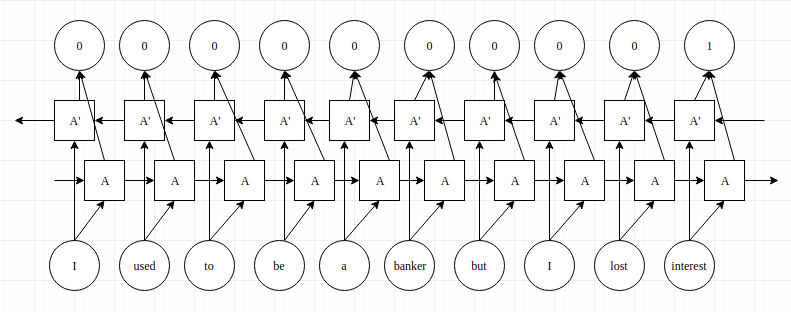
\includegraphics[width=110mm]{figures/lstm.png}
	\caption{Sequence-Labeling Bidirectional LSTM}
	\label{fig:LSTM}
\end{figure}

\subsection{Sliding Window based Maximum Entropy Markov Model}

We implemented a MEMM which tooks a word and a window of words preceding and
following it, as well as a number of features based on that word formed using
feature templates (see table \ref{tab:memm_features}), which output the probability
that that word was a pun or not. We run the algorithm over all words in the
sentence, again treating the problem like a sequence labeling task, and output
as the index of the word in the sentence with the highest probability of being
labeled a pun. Our intuition behind this approach was twofold: 1) it could
handle arbitrary, 2) it could handle arbitrary sentence lengths. 

\begin{table}
\caption{Sliding Window MEMM Features}\label{tab:memm_features} 
\begin{center}
\begin{tabular}{l l} 
\toprule
\textbf{Feature Name} & \textbf{Explanation} \\
\midrule
words\_remaining & number of words after this one \\
lemma            & the lemma, from WordNet \\
shape            & the wordshape \\
prefix3          & first three letters \\
suffix3          & last three letters \\
word             & the word being examined \\
pos              & part of speech \\
stopword         & if the word is a stopword \\
en-wordlist      & if the word is in the english language \\
\bottomrule
\end{tabular}
\end{center}
\end{table}

\subsubsection{Feature Comparision}

We iteratively ran different combinations of features using the Summit
Supercomputer [12] to identify the best set of features to use. 

\begin{figure}[h!]
    \centering
    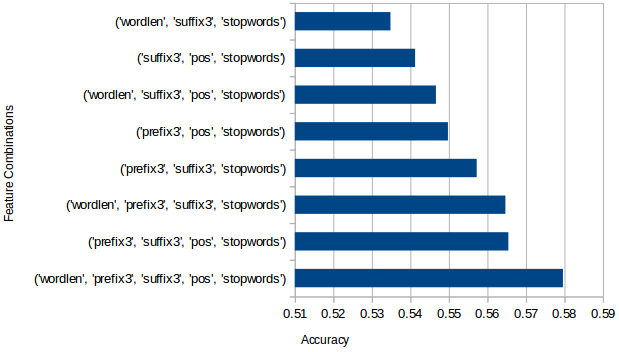
\includegraphics[width=8cm]{figures/sliding_window_homographic.png}
	\caption{Sliding Window MEMM Feature Comparison (Homographic Puns, 40 iterations)}
    \label{fig:method}
\end{figure}

\begin{figure}[h!]
    \centering
    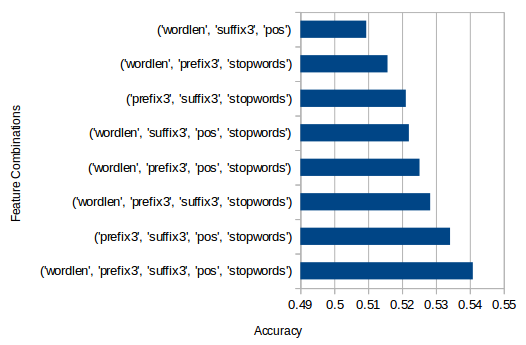
\includegraphics[width=8cm]{figures/sliding_window_heterographic.png}
	\caption{Sliding Window MEMM Feature Comparison (Heterographic Puns, 40 iterations)}
    \label{fig:method}
\end{figure}



\section{Results}\label{results}

\subsection{Evaluation}

We used the same evaluation metrics for each of these tasks were used in
SemEval2017:

\begin{itemize}
	\item{
		\textbf{Pun Detection}: accuracy, precision, recall, F-1
	}
	\item{
		\textbf{Pun Location}: $\frac{correct}{total}$
	}
\end{itemize}

We did quite well on the pun detection tasks, beating the SemEval systems,
particularly for the Heterographic dataset. However, we were not able to best
the SemEval systems for location, with our best accuracy at about $5\%$ below
theirs for homographic and $15\%$ below theirs for heterographic.

\begin{table}
\caption{Pun Detection Results}\label{tab:pun_detection_results}
\begin{center}
\begin{tabular}{l l l l l} 
\toprule
\multicolumn{5}{c}{\textbf{Homographic}}\\
\textbf{Classifier}					& \textbf{Accuracy}	& \textbf{Precision}	& \textbf{Recall}	& \textbf{F-1}\\
Multinomial Naive Bayes (Baseline)	& 0.8043			& 0.8059				& 0.8043			& 0.8051\\
Bidirection LSTM					& 0.8365			& 0.8479				& 0.8365			& 0.8421\\
Feature-Engineered SGD SVM			& 0.8386			& 0.8387				& 0.8386			& 0.8387\\
SemEval2017 Best					& 0.9024			& 0.8970				& 0.8533			& 0.8997\\
\midrule
\multicolumn{5}{c}{\textbf{Heterographic}}\\
\textbf{Classifier}					& \textbf{Accuracy}	& \textbf{Precision}	& \textbf{Recall}	& \textbf{F-1}\\
Multinomial Naive Bayes (Baseline)	& 0.8118			&  0.8119				& 0.8118			& 0.8118\\
Bidirection LSTM					& 0.8160			& 0.8236				& 0.8160			& 0.8198\\
Feature-Engineered SGD SVM			& 0.8179			& 0.8189				& 0.8179			& 0.8184\\
SemEval2017 Best					& 0.8704			& 0.8190				& 0.7837			& 0.8439\\
\bottomrule
\end{tabular}
\end{center}
\end{table}

\begin{table}
\caption{Pun Location Results}\label{tab:pun_location_results}
\begin{center}
\begin{tabular}{l l} 
\toprule
\multicolumn{2}{c}{\textbf{Homographic}}\\
\textbf{Classifier}					& \textbf{Accuracy}\\
Heuristic Decision Tree (Baseline)	& 0.4353\\
Sequence-Labeling Bidirection LSTM	& 0.4517\\
Sliding Window MEMM					& 0.6069\\
SemEval2017 Best					& 0.6631\\
\midrule
\multicolumn{2}{c}{\textbf{Heterographic}}\\
\textbf{Classifier}					& \textbf{Accuracy}\\
Heuristic Decision Tree (Baseline)	& 0.5188\\
Sequence-Labeling Bidirection LSTM	& 0.3745\\
Sliding Window MEMM					& 0.5345\\
SemEval2017 Best					& 0.7964\\
\bottomrule
\end{tabular}
\end{center}
\end{table}



\subsection{Error Analysis}

In order to help better detect puns correctly, we looked at when sentences were falsely being detected as containing puns, as well as when sentences with puns were classified as non-puns. Looking at it in this way, we could better understand where we needed to improve and which types of features might be useful to help better distinguish puns. This required looking at the output for sentences to see if they were correctly being identified, or if our classifiers were giving errors. The web app we created was actually pretty useful for this purpose as it allowed us to easily enter sentences one by one and look at output for different classifiers. For example, one thing we noticed was that many cases, sentences with idioms were incorrectly being identified as sentences with puns. To alleviate this problem, an idiom feature was added. Another metric that helped in error analysis of our pun detection was looking at a confusion matrix for when we had false positives or negatives and seeing in which direction we were most likely to be incorrect. We also looked at number of epochs used in some of our classifiers to determine if we were overfitting on data during training, and tuned the number of epochs used to most accurately classify puns. At one point, we noticed we were getting 100\% training accuracy, which signified we were likely overfitting on the training set.

Other techniques we used throughout development were useful as well in error analysis. For example, feature comparison was helpful as we could see which features were helping or hurting accuracy, and analyze why sentences containing those features might be classified incorrectly. For example in bigrams feature, if the bigram "lost interest" was found in a sentence containing a pun, the next time a sentence appeared with that same bigram, that sentence might also be classified as a pun. However, that is generally not the case that "lost interest" would be found in a sentence containing a pun. However, due to the infrequency of this bigram in our dataset, all other sentences with this bigram might be incorrectly identified if they did not contain puns. 

In addition to analyzing errors in pun detection, we analyzed the accuracy of our location pun-classifiers as a function of
sentence length. In general, the smaller the sentence length, the more accurate
the classifier. In particular, it can be seen that the MEMM retains more of its
accuracy on longer sentences, while the Bidirectional LSTM drops significantly. 
A possible way to address this would be to give the LSTM an attention model, but
we unfortunately were unable to implement this.

\begin{figure}[h!]
    \centering
    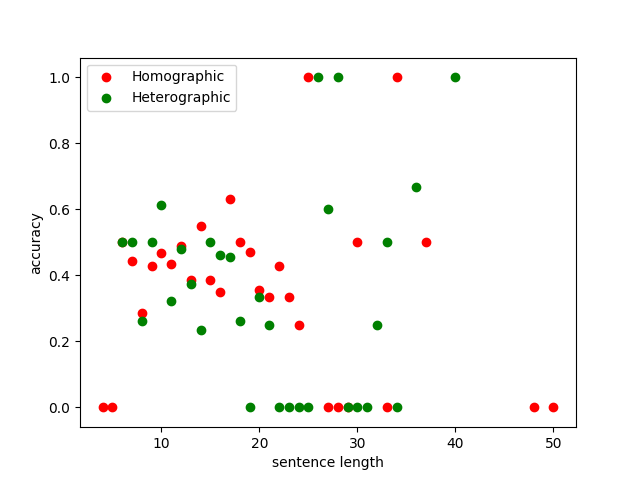
\includegraphics[width=8cm]{figures/location-rnn.png}
	\caption{Bidirectional LSTM accuracy as a function of sentence length}
    \label{fig:method}
\end{figure}

\begin{figure}[h!]
    \centering
    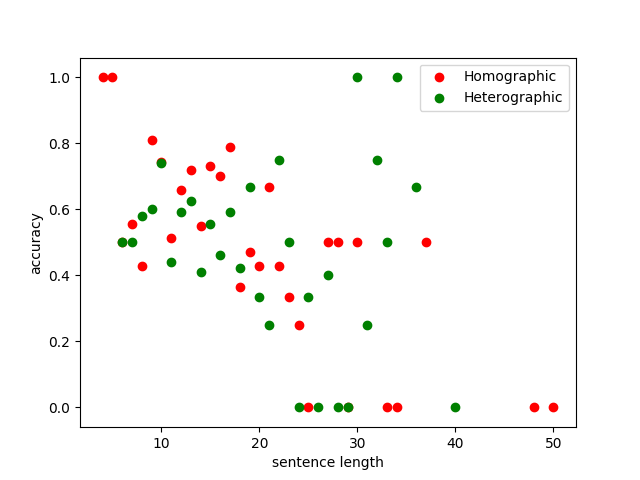
\includegraphics[width=8cm]{figures/location-window.png}
	\caption{Sliding Window MEMM accuracy as a function of sentence length}
    \label{fig:method}
\end{figure}


\subsection{Motivation for Approaches}
Much of our inspiration for this project came from SemEval 2017. However, many of the systems in SemEval did not leverage machine learning approaches, which is why we felt using machine learning for the task would be an interesting approach. As we began this project, we tried adding in several classifiers as we wanted to see how they varied in performance. Then, by looking at the errors in these classifiers, cross-validation, feature comparison, and through further research, we were able to test out different ideas to  improve upon our first attempts at these classifiers. 

Much of our ideas for features to add came through various intuitions about the nature of sentences containing puns. For example, our most useful feature, which relied on nltk's lesk algorithm and looked at word distances, came from the idea that the pun word might be pretty different, or seemingly out-of-place, from the other words in the sentence.  

When looking at pun location, we needed to find algorithms that would be able to handle various sentence lengths and also look at each word individually. We also felt that this task could be seen as a sequence labeling task, and looked at algorithms that would enable us to do that. 

Most of the ideas for choice of classifiers came from looking at their architecture and seeing how it would be helpful for our problem. More specifics about the approaches for each classifier individually can be found in their respective sections.



\subsection{Cross Validation}
In addition to creating these classifiers, we also needed to tune various hyperparameters used in order to get the best results possible. We found Scikit-learn's GridSearchCV function useful for k-fold cross validation to compare different values. We also ran each combination of parameters multiple times to get average values for accuracy for each run. From these results, we were able to incorporate better default values of different parameters in our classifiers. 

\subsection{Applications}
We were able to use our classifiers to put together a web application to allow users to enter sentences and see different classifiers' results about them. The application can give information as to whether or not a sentence contains a pun, which type of pun the sentence is most likely to contain, and the word in the sentence most likely to be a pun, with more likely words shown in a darker color. This application is publicly available at ec2-54-165-55-37.compute-1.amazonaws.com.

%%%%%%%%%%%%%%%%%%%%%%%%%%%%%%%%%%%%%%%%%%%%%%%%%%%%%%%%%%%%%%%%%%%%%%%%%%%%%%%
% Conclusion
%%%%%%%%%%%%%%%%%%%%%%%%%%%%%%%%%%%%%%%%%%%%%%%%%%%%%%%%%%%%%%%%%%%%%%%%%%%%%%%

\section{Conclusion}
\label{conclusion}

\subsection{What Went Well}

We did well at pun detection, largely leveraging the size of our dataset over
what the systems at SemEval had access to. We also were fairly successful in
trying different algorithms and evaluating combinations of different features. 

\subsection{What We Could Have Done Better}

The best systems at SemEval applied different approaches to the problem for the
two types of data, heterographic and homographic. This makes sense, as the
characteristics of those two datasets differ significantly. Generally, our
approach would have benefited from adding more information to our attempts at
the heterographic dataset, perhaps converting the words in a sentence into their
phonemes and identifying possible words which were close in sound.

We also worked on a few other classifiers that we did not have time to fully complete and evaluate, and hence are not included in the report. We added a voting classifier to ensemble the results of other classifiers, and do a majority vote on the predictions from each classifier used. Preliminary results showed this classifier was actually in some cases performing poorly as it was incorporating results from all classifiers, even baseline. Either weighting the results for each of the classifiers based on their accuracy or writing and adding in more classifiers to the voting classifier may have been helpful. It also would have been interesting to try boosting techniques like Adaboost, and we attempted to add this to our sliding window classifier, but we did not have enough time to get final results and do analysis on this method.

We also could have improved in looking at error analysis. Getting a list of sentences misclassified, either negatively or positively, and looking at general trends in those errors (like maybe all the false positives are long sentences, for example), would have been extremely useful in better coming up with features and classifiers more likely to classify these sentences correctly. While we looked at sentences more on an individual basis with errors and were able to get a few intuitions about them, looking at the misclassified sentences as a group would have been even better. If we had more time on this project, this would be a wonderful next step.

\subsection{Future Work}

An obvious shortcoming of our system is that it will only predict \emph{one
word} as the pun word, but, and the idea that there is \emph{one word} the makes
a pun is somewhat dubious (not to mention that compound puns exist). Consider
the following pun: 
\begin{center}
	\emph{The rabbi got hit on the temple.}
\end{center}
Our system would say that the punword is ``temple'', but that is really only half
the story; if the word ``rabbi'' were replaced with, say, ``monk'', there would
be no pun. The ability to identify the words \emph{involved} in a pun would be
much more useful, and to the authors of this report, more interesting.

Of obvious interest is the ability to detect further types of puns, perhaps
using context provided by different types of data; it would be extremely
interesting to create a system which could identify visual puns. 

It would be of interest to say \emph{what} about the words in a sentence make it
a pun. In other words, the creation of a system which could interpret puns.

A more out-there hope would be a system which could generate puns, perhaps being
given a sentence and a pair of word senses.

\subsection{Who Did What}

Project Github Repository: \url{https://github.com/hunter-/pun_classifier}

\begin{itemize}
\item Shantanu Karnwal worked on:
	\begin{itemize}
		\item decision tree classifier for pun location
		\item feature comparison for the sliding window MEMM
		\item poster layout and content
		\item report content (pun location images)
	\end{itemize}
\item Amir Kashipazha
	\begin{itemize}
		\item features (antonyms, idioms, sentiment)
		\item feature comparison for the SVM used for SGD Pun Detection
		\item report content (feature comparison for the SVM used for SGD Pun Detection)
		\item final benchmarks of classifiers
	\end{itemize}
\item Brandon Boylan-Peck
	\begin{itemize}
		\item poster bar graphs
	\end{itemize}
\item Cathlyn Stone
	\begin{itemize}
		\item interactive web app
		\item framework for running classifiers
		\item features (lesk algorithm, POS, Tfidf)
		\item SVM used in the SGD Pun Detection algorithm
		\item sliding window MEMM used in Pun Location
		\item ensemble algorithm
		\item algorithm cross validation
		\item Bidirectional LSTM used for Pun Location
		\item evaluation of the Pun Detection algorithms
		\item model caching architecture
		\item report content 
		\item error analysis
	\end{itemize}
\item Kenneth Hunter Wapman
	\begin{itemize}
		\item data loading and manipulation
		\item baseline algorithm for Pun Detection
		\item features (word embeddings)
		\item framework for running classifiers
		\item sliding window MEMM used in Pun Location
		\item Bidirectional LSTM used for Pun Location
		\item Bidirectional LSTM used for Pun Detection
		\item evaluation of the Pun Location algorithms
		\item poster content
		\item report content
		\item error analysis
	\end{itemize}
\end{itemize}

\subsubsection*{Acknowledgments}

We were helped immeasurably by the systems described in SemEval2017. Tyler
Scott's advice on LSTMs was also extremely helpful. We also thank this semester's course in machine learning in giving us valuable insight into these algorithms and allowing us to understand this vast area of computer science more deeply.

%%%%%%%%%%%%%%%%%%%%%%%%%%%%%%%%%%%%%%%%%%%%%%%%%%%%%%%%%%%%%%%%%%%%%%%%%%%%%%%
% References
%%%%%%%%%%%%%%%%%%%%%%%%%%%%%%%%%%%%%%%%%%%%%%%%%%%%%%%%%%%%%%%%%%%%%%%%%%%%%%%
\section*{References}

\medskip

\small

[1] Oele, D., \& Evang, K.\ (2017) BuzzSaw at SemEval-2017 Task 7:
Global vs. Local Context for Interpreting and Locating Homographic English Puns
with Sense Embeddings. Proceedings of the 11th International Workshop on
Semantic Evaluations (SemEval-2017), pages 444–448, Vancouver, Canada, August 3
- 4, 2017. 2017 © Association for Computational Linguistics.

[2] Pedersen, T.\ (2017) Duluth at SemEval-2017 Task 7: Puns Upon a Midnight
Dreary, Lexical Semantics for the Weak and Weary. Proceedings of the 11th
International Workshop on Semantic Evaluations (SemEval-2017), pages 416–420,
Vancouver, Canada, August 3 - 4, 2017. 2017 © Association for Computational
Linguistics.

[3] Xiu, Y., Lan, M., \& Wu, Y.\ (2017). ECNU at SemEval-2017 Task 7: Using
Supervised and Unsupervised Methods to Detect and Locate English Puns.
Proceedings of the 11th International Workshop on Semantic Evaluations
(SemEval-2017), pages 453–456, Vancouver, Canada, August 3 - 4, 2017. 2017 ©
Association for Computational Linguistics.

[4] Hurtado, L., Segarra, E., Pla, F., Carrasco, P., \& Gonzalez, J.A..
(2017). ELiRF-UPV at SemEval-2017 Task 7: Pun Detection and Interpretation.
Proceedings of the 11th International Workshop on Semantic Evaluations
(SemEval-2017), pages 440–443, Vancouver, Canada, August 3 - 4,
2017. 2017 © Association for Computational Linguistics.

[5] Indurthi, V., \&  Reddy, O.S.\ (2017). Fermi at SemEval-2017 Task
7: Detection and Interpretation of Homographic puns in English Language.
Proceedings of the 11th International Workshop on Semantic Evaluations
(SemEval-2017), pages 457–460, Vancouver, Canada, August 3 - 4, 2017. 2017 ©
Association for Computational Linguistics.

[6] Samuel Doogan, Aniruddha Ghosh, Hanyang Chen, and Tony Veale. 2017. Idiom
Savant at Semeval-2017 Task 7: Detection and Interpretation of English Puns.
Proceedings of the 11th International Workshop on Semantic Evaluations
(SemEval-2017), pages 103–108, Vancouver, Canada, August 3 - 4, 2017. 2017 ©
Association for Computational Linguistics.

[7] Das, D. \& Pramanick, A. (2017). JU\_CSE\_NLP at SemEval 2017 Task 7:
Employing Rules to Detect and Interpret English Puns. Proceedings of the 11th
International Workshop on Semantic Evaluations (SemEval-2017), pages 432–435,
Vancouver, Canada, August 3 - 4, 2017. 2017 © Association for Computational
Linguistics.

[8] Mikhalkova, E. \& Karyakin, Y. (2017). PunFields at SemEval-2017 Task 7:
Employing Roget’s Thesaurus in Automatic Pun Recognition and Interpretation.
Proceedings of the 11th International Workshop on Semantic Evaluations
(SemEval-2017), pages 426–431, Vancouver, Canada, August 3 - 4, 2017. 2017 ©
Association for Computational Linguistics.

[9] Bahuleyan, H. \& Vechtomova, O. (2017). UWaterloo at SemEval-2017 Task 8:
Detecting Stance towards Rumours with Topic Independent Features. Proceedings
of the 11th International Workshop on Semantic Evaluations (SemEval-2017),
pages 461–464, Vancouver, Canada, August 3 - 4, 2017. 2017 © Association for
Computational Linguistics.

[10] Vadehra, A. (2017). UWAV at SemEval-2017 Task 7: Automated feature-based
system for locating puns. Proceedings of the 11th International Workshop on
Semantic Evaluations (SemEval-2017), pages 449–452, Vancouver, Canada, August 3
- 4, 2017. 2017 © Association for Computational Linguistics.

[11] Sevgili, O., Ghotbi, N., \& Tekir, S. (2017). N-Hance at SemEval-2017 Task
7: A Computational Approach using Word Association for Puns. Proceedings of the
11th International Workshop on Semantic Evaluations (SemEval-2017), pages
436–439, Vancouver, Canada, August 3 - 4, 2017. 2017 © Association for
Computational Linguistics.

[12] Jonathon Anderson, Patrick J. Burns, Daniel Milroy, Peter Ruprecht, Thomas Hauser, and Howard Jay Siegel. 2017. Deploying RMACC Summit: An HPC Resource for the Rocky Mountain Region. In Proceedings of PEARC17, New Orleans, LA, USA, July 09-13, 2017, 7 pages. DOI: 10.1145/3093338.3093379

\end{document}
